\documentclass[12pt,graphicx,caption,rotating]{article}
\textheight=23cm
\textwidth=17cm
\topmargin=-1cm
\oddsidemargin=0cm
\usepackage[activeacute,spanish]{babel}
\usepackage[utf8]{inputenc}
\usepackage{graphicx}%manejo de graficos
\usepackage{times}
\usepackage{amssymb,amsfonts}
\usepackage[tbtags]{amsmath}
\usepackage{cite}
\usepackage[all]{xy}
\usepackage{subfigure}
\usepackage{wrapfig}
\usepackage{color}
\usepackage{multicol}
\usepackage{cite}
\usepackage{url}
\usepackage[tbtags]{amsmath}
\usepackage{amsmath,amssymb,amsfonts,amsbsy}
\usepackage{bm}
\usepackage{algorithm}
\usepackage{algorithmic}
\usepackage[all]{xy}
\usepackage[centerlast, small]{caption}
\usepackage[colorlinks=true, citecolor=blue, linkcolor=blue, urlcolor=blue, breaklinks=true]{hyperref}
\hyphenation{ele-men-tos he-rra-mi-en-ta cons-tru-yen trans-fe-ren-ci-a pro-pu-es-tas si-mu-lar vi-sua-li-za-cion}

\begin{document}

\title{\textbf{Práctica 1:} Porcentaje de modulación de una señal modulada en amplitud con portadora de alta potencia y medición del espectro de frecuencia de la señal modulada}
\author{Juan Carlos Cabrera Cardenas \textbf{Código:} $258197$ \href{juccabreraca@unal.edu.co}{juccabreraca@unal.edu.co} \\
      Diego Alexander Huerfano Villalba \textbf{Código:} $258267$ \href{dahuerfanov@unal.edu.co}{dahuerfanov@unal.edu.co}\\
      David Ricardo Martínez Hernández \textbf{Código:} $261931$ \href{drmartinezhe@unal.edu.co}{drmartinezhe@unal.edu.co}}
\date{}
\maketitle

\begin{table}[H]
  \centering
  \caption{Porcentaje de modulación con señal modulante interna y sin circuito de carga.}
    \begin{tabular}{|c|c|c|c|c|} \hline
      Valor medido de la & Valor medido de la  & $M_{1}$ $\%$ & $M_2$ $\%$ & $M_3$ $\%$ \\
      señal $E_{max}$ & señal $E_{min}$ &  &  & \\ \hline
      $4$ & $4$ & $0$ & $0$ & $0$ \\ \hline
      $5$ & $2.93$ & $141.54$ & $41.54$ & $26.1$ \\ \hline
      $6$ & $1.97$ & $48.88$ & $51.11$ & $50.56$ \\ \hline
      $7$ & $1.13$ & $19.25$ & $80.75$ & $72.2$ \\ \hline
      $8$ & $0$ & $0$ & $100$ & $100$ \\ \hline
    \end{tabular}
  \label{tab1}
\end{table}

\begin{table}[H]
  \centering
  \caption{Valores de frecuencias.}
   \begin{tabular}{|c|c|c|}\hline
    Frecuencia de la portadora & Frecuencia de la señal& Frecuencia de la señal \\
    &  lateral superior & lateral inferior \\ \hline
    $10.052$ $KHz$ & $10.4089$ $KHz$ & $9.6049$ $KHz$ \\ \hline
    \end{tabular}
  \label{tab2}
\end{table}

\begin{table}[H]
  \centering
  \caption{Amplitudes espectrales.}
    \begin{tabular}{|c|c|c|c|c|} \hline
      Valor medido de la & Valor medido de la & Amplitud espectral & Amplitud espectral & Amplitud espectral \\
      señal $E_{max}$ (V) & señal $E_{min}$ (V) & de la portadora & de la señal lateral & de la señal lateral \\
      &  & modulada (dB) & superior (dB) & inferior (dB) \\ \hline
      $4$ & $4$ & $9.01$ & $0$ & $0$ \\ \hline
      $5$ & $2.64$ & $8.65$ & $-6.95$ & $-7.35$ \\ \hline
      $6$ & $1.68$ & $9.05$ & $-2.15$ & $-2.15$ \\ \hline
      $7$ & $0.68$ & $8.23$ & $-0.169$ & $-0.169$ \\ \hline
      $8$ & $0.16$ & $7.83$ & $1.43$ & $1.43$ \\ \hline
    \end{tabular}
  \label{tab3}
\end{table}

\begin{figure}
  \centering
   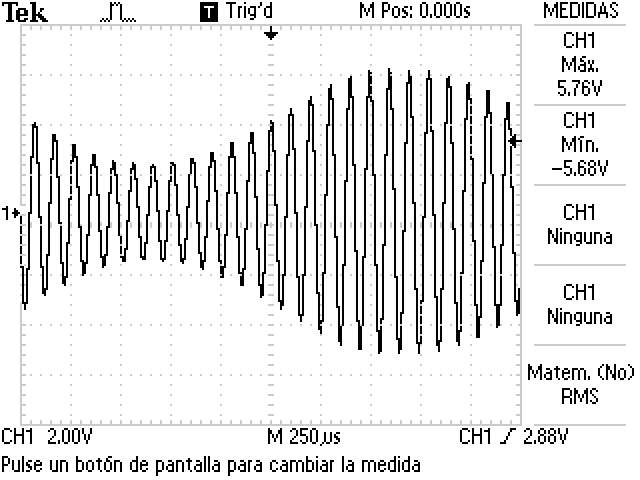
\includegraphics[scale=0.5]{fig1.jpg}
    \caption{Señal Modulada obtenida en el osciloscopio con un $\mu$=50\%.}
  \label{fig1}
\end{figure}

\begin{figure}
  \centering
    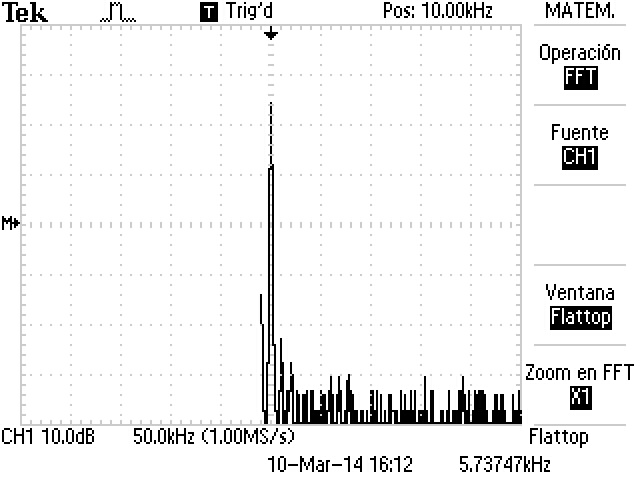
\includegraphics[scale=0.5]{fig2.jpg}
    \caption{Representación espectral obtenida en el osciloscopio.}
  \label{fig2}
\end{figure}

\begin{figure}
  \centering
    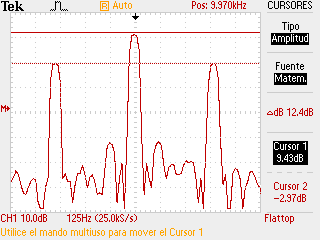
\includegraphics[scale=1]{fig3.png}
    \caption{Representación espectral obtenida en el osciloscopio de la señal con un índice de modulación de $\mu = 50 \%$.}
  \label{fig3}
\end{figure}

\section*{Conclusiones}
\begin{itemize}
 \item Como se puede observar en los archivos adjuntados las ganancias obtenidas del analizador de espectros de Multisim, no son las mismas en las diferentes configuraciones suponemos que es debido a las pérdidas que tiene el simulador de forma intrínseca, porque matemáticamente las funciones son las mismas, la única diferencia es que se han añadido una mayor cantidad de cables y de fuentes.
 
 \item A medida que se varía el índice de modulación $\mu$, se pudo observar como la señal modulada cambiaba su forma, es decir desde tener una envolvente senoidal la cual cruzaba por cero con $\mu=100$ hasta una envolvente constante con $\mu=0$, además se pudo observar como varían las amplitudes de la señal lateral superior e inferior.
 
 \item Se evidenció claramente de acuerdo a los resultados  teóricos desarrollados en clase tanto la presencia como su valor en amplitud espectral de las frecuencias laterales que surgen en el proceso de modulación.
\end{itemize}
\end{document}